% !TEX root = ../report.tex
\chapter{Einleitung}
\begin{Spacing}{\mylinespace}
\begin{figure}[h!]
	\centering
	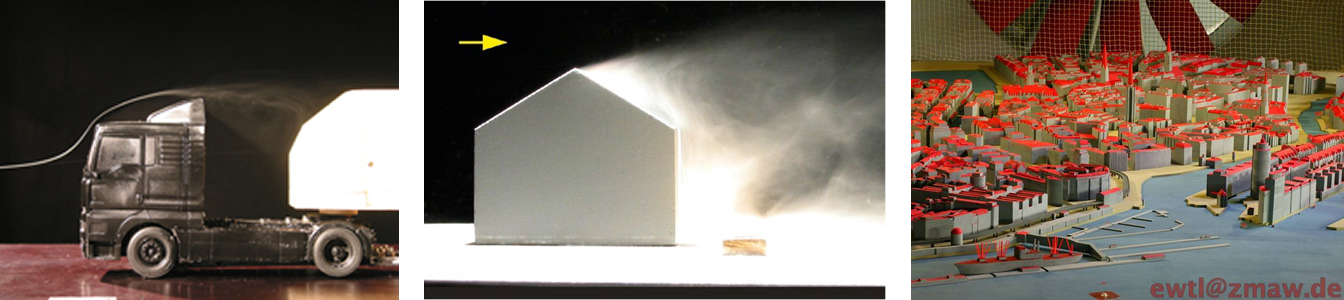
\includegraphics[width=\textwidth]{graphics/intro.png}
\end{figure}
Die Technik der Strömungssimulation spielt heutzutage eine größere Rolle den je. Lange ist es her das Windkanäle nur zur Erforschung und Verbesserung der Aerodynamik von Flugzeugen genutzt wurde. Heute gibt es kaum noch ein Kraftfahrzeug das nicht im Windkanal optimiert wurde und auch Architekten und Statiker nutzen immer häufiger den Windkanal um ihre Konstruktionen und Berechnungen zu überprüfen. Ein relativ neues Thema in diesem Gebiet ist die Untersuchung kompletter Stadtteilen und Städten im Windkanal. Durch den enormen Anstieg von neuen Wohn-, Gewerbe- und Industriegebieten in den letzten Jahrzehnten, schrumpft der Anteil von freien und natürlichen Flächen immer weiter, wodurch die Frischluftzufuhr negativ beeinflusst wird und sich das Klima in Städten stetig weiter erwärmt und verschlechtert. Um dieser Entwicklung entgegen zu wirken nutzen auch Städteplaner immer häufiger die Vorzüge des Windkanals.
\\\\
So nützlich der Windkanal auch für alle vorgestellten Anwendungen ist, so ist dessen Nutzung auch immer mit sehr hohen Kosten verbunden. Durch die immer weiter steigende Leistung von Computern liegt es deshalb nahe, zu versuchen, erste Tests und Untersuchung von der Realität auf den Computer auszulagern und auf diesem zu simulieren. Genau aus diesem Gebiet bestand der Hauptteil unserer Forschung in diesem Semester. Um dieses doch sehr mathematische und trockene Thema für Außenstehende noch etwas attraktiver und greifbarer zu machen haben wir es jedoch, mit Hilfe der Kinect Kamera von Microsoft, noch um eine Interaktive Komponente erweitert.
\\\\
Auf den Folgenden Seiten werden wir nun unser Vorgehen sowie die Fortschritte, Erfahrungen und Ergebnisse dieses Projekts vorstellen.
\end{Spacing}
\newpage
\clearpage
%% End Of Doc